% =============================================================================
% sections/design/safety/emergency_stop.tex  -  Emergency Stop
% Teams: electronics + software (best guess - unconfirmed) / Status: stub
%
% Nested under "Safety Systems" (section-level subsection).
% =============================================================================

\begin{figure}[H]
    \centering
    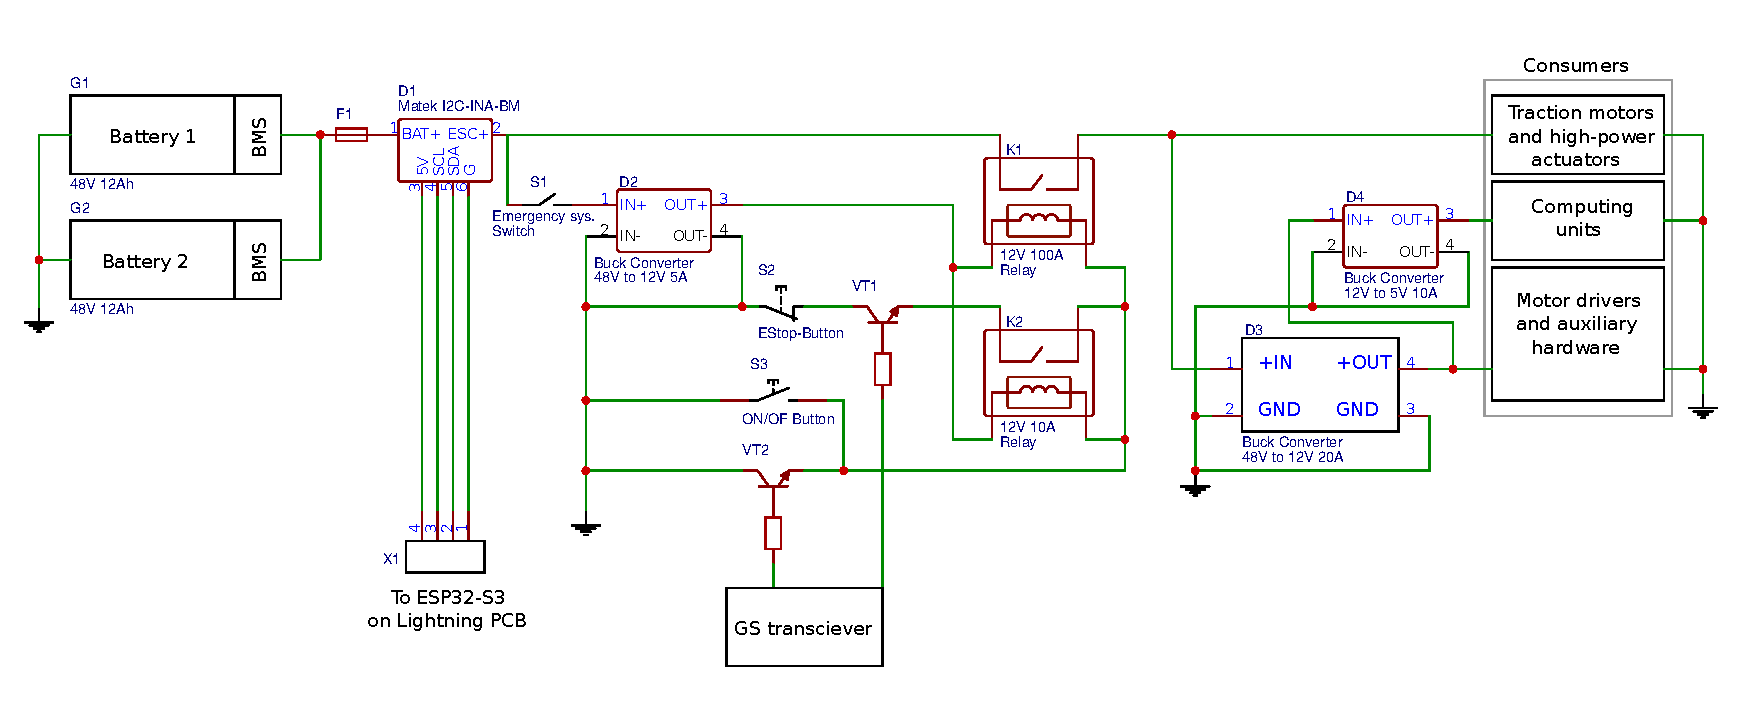
\includegraphics[width=\linewidth]{teams/electronics/figures/hardware_safety.pdf}
    \caption{Electrical schematic of the rover hardware safety system.}
    \label{fig:hardware_safety}
\end{figure}

The rover uses a dedicated hardware safety system independent of the main control electronics (Fig. \ref{fig:hardware_safety}). The primary power path is protected by a fuse (F1), while an INA-based module (D1) monitors battery voltage and current for state estimation and fault detection.

Power switching is implemented as a hardware self-latching circuit using relays K1 and K2, supplied by an independent 48 V-to-12 V converter (D2). The rover is powered on via the ON/OFF button (S3) or a remote command, while the relays maintain the powered state until an emergency stop is triggered.

Emergency shutdown can be triggered locally via the E-Stop button (S2) or remotely through an independent wireless channel. Both interrupt the relay latching circuit, immediately disconnecting rover power. As the emergency stop is implemented entirely in hardware, it operates independently of the onboard computer and software.

Rover status is indicated by a 360° industrial signal lamp mounted at its highest point. Four colors represent the operating state: orange (power on), green (manual mode), red (autonomous mode), and blue (wireless connection established).

The electronics enclosure is sealed with dedicated covers for removable modules, reducing dust and water ingress while ensuring reliable outdoor operation.

